\documentclass[handout]{beamer}

\usepackage{Haust2017glærur}

\title{Stærðfræðimynstur í tölvunarfræði}
\subtitle{Vika 3, fyrri fyrirlestur}

\begin{document}

\begin{frame}
\titlepage
\end{frame}

\section{Inngangur}

\begin{frame}{Í síðasta tíma}
\begin{itemize}
 \item Mengi!
 \begin{itemize}
  \item Stök í mengjum
  \item Hlutmengi
  \item Veldismengi og mengjamargfeldi
  \item Sniðmengi og sammengi
 \end{itemize}
 \item Föll 
\end{itemize}
\end{frame}

\section{Runur (2.4)}

\begin{frame}{Runur}
\begin{tcolorbox}[title=Runur]
Runa (e. \emph{sequence}) er fall frá hlutmengi heiltalna (oftast mengi jákvæðra heiltalna) til annars mengis $S$. Mynd heiltölunnar $n$ er táknuð með $a_n$. Sagt er að $a_n$ sé liður (e. \emph{term}) í rununni.
\end{tcolorbox}
Bókin táknar runur með slaufusvigum, t.d. $\{a_n\}$. Runur eru samt ekki mengi.

Dæmi um runu:
\[
 \{a_n\} = a_1, a_2, a_3 \ldots = 1, \frac{1}{2}, \frac{1}{3}
\]
\[
 a_n = \frac{1}{n}
\]
\end{frame}

\begin{frame}{Kvótarunur}
    \begin{tcolorbox}[title=Kvótarunur]
        Kvótaruna (e. \emph{geometric progression}) er runa á sniðinu
        \[
            a, ar, ar^2, \ldots, ar^n, \ldots
        \]
        þar sem $a$ og $r$ eru rauntölur.
    \end{tcolorbox}
    Hér er \emph{hlutfall} hverra tveggja aðlægra liða jafnt.

    \vspace{0.5cm}
    Kvótarunum svipar til vísisfallsins $f(x) = ar^x$
\end{frame}

\begin{frame}{Kvótarunur}
    \begin{columns}
        \column{0.5\textwidth}
        \begin{itemize}
            \item Kvótarunur koma oft upp í rúmfræði
            \item Til vinstri: Röð ferninga
            \begin{itemize}
                \item Flatarmál ferninganna má tákna með runu:
                \[
                    \frac{1}{4}, \frac{1}{16}, \frac{1}{64}
                \] 
            \end{itemize}
            \item Summa allra liða raðarinnar er $\frac{1}{3}$
        \end{itemize}
        \column{0.5\textwidth}
        \begin{center}
            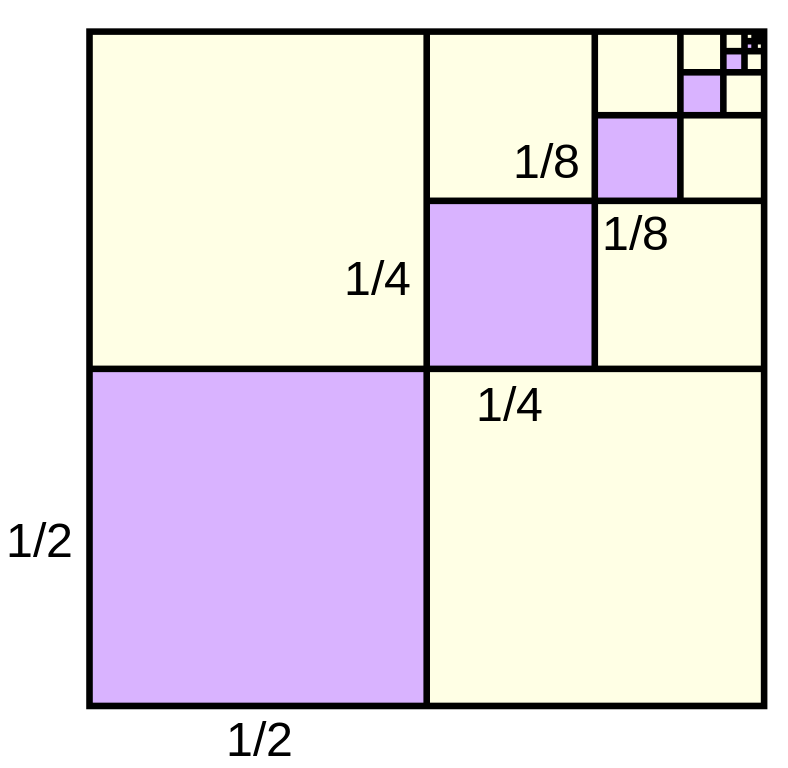
\includegraphics[width=\textwidth]{geometric-squares}

            Mynd: \href{https://en.wikipedia.org/wiki/File:GeometricSquares.svg}{Wikipedia}.
        \end{center}
    \end{columns}
\end{frame}

\begin{frame}{Jafnmunaruna}
    \begin{tcolorbox}[title=Jafnmunaruna]
        Jafnmunaruna (e. \emph{arithmetic progression}) er runa á sniðinu
        \[
            a, a+d, a+2d, \ldots, a + nd, \ldots
        \]
        þar sem $a$ og $d$ eru rauntölur.
    \end{tcolorbox}
\end{frame}

\begin{frame}[fragile]{Strengir}
\begin{itemize}
 \item Sérstök, mikið notuð gerð af runum kallast strengur (e. \emph{string})
 \item Strengur er endanleg runa af stöfum, úr endanlegu mengi (stafrófinu)
 \begin{itemize}
  \item Stafrófið getur verið hvaða mengi sem er, en algeng stafróf eru \texttt{\{'a', 'b', 'c', \ldots\}} og \texttt{\{0, 1\}}
 \end{itemize}
\end{itemize}

\begin{minted}[frame=lines]{java}
// Gagnagerðin String í Java í notkun
String s = "Ég er strengur!";
String b = "01010110";
\end{minted}
\end{frame}

\begin{frame}{Strengir}
    \begin{itemize}
        \item Strengir eru nógu mikið notaðir til að fá sérstaka, stutta rithætti
        \begin{itemize}
            \item Í stærðfræði eru táknin talin upp: $abcd$
            \item Í forritunarmálum eru strengir oftast afmarkaðir með gæsalöppum: \textbf{"abcd"}
        \end{itemize}
        \item Lengd strengs er fjöldi tákna sem í honum eru
        \item Tómi strengurinn $\lambda$ inniheldur engin tákn og er af lengdinni 0
    \end{itemize}
\end{frame}

\begin{frame}{Summur}
    Algengt er að leggja saman liði í runu. Samlagning á liðunum $a_m, a_{m+1}, \ldots, a_n$ í röð $\{a_n\}$ er táknuð með

    \[
        \sum_{j=m}^n a_j = a_m + a_{m+1} + \ldots + a_n
    \]
    Hægt er að tala um ``summu frá $m$ til $n$''.
\end{frame}

\begin{frame}{Rakningarvensl}
\begin{tcolorbox}[title=Rakningarvensl]
Rakningarvensl (e. \emph{recurrence relation}) fyrir runu $\{a_n\}$ er jafna sem skilgreinir $a_n$ sem fall af einum eða fleiri fyrri liðum rununnar, þ.e.a.s. $a_0, a_1, \ldots, a_{n-1}$ fyrir öll $n > n_0$, þar sem $n_0$ er ekki-neikvæð heiltala.
\end{tcolorbox}
Runa er lausn (e. \emph{solution}) á rakningarvenslum ef liðir hennar uppfylla venslin. Liðirnir sem eru fyrir framan fyrsta liðinn sem rankningarvenslin tilgreina eru upphafsskilyrði (e. \emph{initial conditions}) þeirra.
\end{frame}

\begin{frame}{Dæmi um rakningarvensl}
Látum $\{a_n\}$ vera runu sem uppfyllir $a_n = a_{n-1} + 3$ fyrir $n=1, 2, 3, \ldots$ og setjum $a_0 = 2$. Hvað eru þá $a_1, a_2$ og $a_3$? \pause

\begin{align*}
a_1 &= a_0 + 3 = 2 + 3 = 5\\
a_2 &= 5 + 3 = 8\\
a_3 &= 8 + 3 = 11\\
\end{align*}

\end{frame}

\begin{frame}{Dæmi um rakningarvensl}
    \begin{columns}
        \column{0.5\textwidth}
        \begin{itemize}
            \item Fibonacci-rununa $f_0, f_1, f_2, \ldots$ má skilgreina með rakningarvenslum
            \begin{itemize}
                \item Upphafsskilyrði: $f_0 = 0, f_1 = 1$
                \item Rakningarvensl: $f_n = f_{n-1} + f_{n-2}$
            \end{itemize}
        \end{itemize}
        \column{0.5\textwidth}
        Hver er 6. Fibonacci talan? \pause
        \begin{align*}
            f_2 &= f_0 + f_1 = 0 + 1 = 1\\
            f_3 &= f_1 + f_2 = 1 + 1 = 2\\
            f_4 &= f_2 + f_3 = 1 + 2 = 3\\
            f_5 &= f_3 + f_4 = 2 + 3 = 5\\
            f_6 &= f_4 + f_5 = 3 + 5 = 8\\
        \end{align*}
    \end{columns}
\end{frame}

\begin{frame}{Að leysa rakningarvensl}
\begin{itemize}
    \item Oft er nauðsynlegt að finna formúlu fyrir liði runu sem skilgreind er með rakningarvenslum
    \begin{itemize}
        \item Slík formúla er kölluð lausn á rakningarvenslunum
    \end{itemize}
    \item Formúlan er sögð vera á lokuðu sniði (e. \emph{closed form}) ef hún inniheldur einungis einfaldar grunnaðgerðir og föll
    \item Algengt: Giska á rétta formúlu, sem síðan er sannreynd með þrepun (e. \emph{induction})
    \begin{itemize}
        \item Gerum meira af því síðar
    \end{itemize}
\end{itemize}
\end{frame}

\begin{frame}{Dæmi um rakningarvensl með lausn}
    Leggjum 10,000\$ inn á bankareikning með 11\% vöxtum sem reiknaðir eru árlega. Hver verður upphæðin á bankareikningnum eftir 30 ár?
    \pause
    Setjum upp rakningarvensl, setjum $P_0 = 10,000$:
    \[
        P_n = P_{n-1} + 0.11P_{n-1} = (1.11)P_{n-1}
    \]
\end{frame}

\begin{frame}{Dæmi um rakningarvensl með lausn}
    Reiknum:
    \begin{align*}
        P_1 &= (1.11)P_0\\
        P_2 &= (1.11)P_1 = (1.11)^2P_0\\
        P_3 &= (1.11)P_2 = (1.11)^3P_0\\
        &\vdots\\
        P_n &= (1.11)P_{n-1} = (1.11)^nP_o\\
    \end{align*}
    Þá er $P_{30} = (1.11)^{30}10,000\$ = 228,922.97\$ $
\end{frame}

\section{Fjöldatölur og reiknanleiki (2.5)}

\begin{frame}{Fjöldatölur}
Við höfum áður kynnst fjöldatölum. Útvíkkum nú hugtakið:

\begin{tcolorbox}[title=Eins fjöldatölur]
Mengin $A$ og $B$ hafa sömu fjöldatölu ef til er gagntækt fall frá $A$ til $B$.
\end{tcolorbox}

\pause Þá má einnig skilgreina:

\begin{tcolorbox}[title=Teljanleiki]
Mengi sem er endanlegt eða hefur sömu fjöldatölu og mengi jákvæðra heiltalna er teljanlegt (e. \emph{countable}). Þegar óendanlegt mengi $S$ er teljanlegt skilgreinum við fjöldatölu þess sem $|S| = \aleph_0$.
\end{tcolorbox}
\end{frame}

\begin{frame}{Dæmi um óendanlegt teljanlegt mengi}
    Jákvæðu oddatölurnar eru teljanlegar:
    
    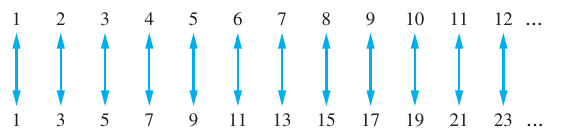
\includegraphics[width=\textwidth]{odd-positives-countable}
    
    Hér er gagntæka fallið fallið $f(n) = 2n-1$.
\end{frame}

\begin{frame}{Ræðu tölurnar eru teljanlegar}
    \begin{columns}
        \column{0.3\textwidth}
        Gæti komið á óvart: við getum skrifað ræðu tölurnar upp í runu með því að fylgja hornalínum
        \column{0.7\textwidth}
        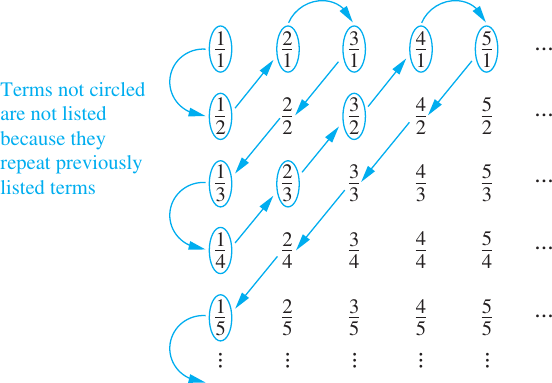
\includegraphics[width=\textwidth]{rational-countable}
    \end{columns}
\end{frame}

\begin{frame}{Reiknanleiki}
\begin{itemize}
 \item Til að fall sé reiknanlegt (e. \emph{computable}) þarf að vera til forrit í einhverju forritunarmáli sem finnur gildi þess
 \item Til eru óreiknanleg föll!
 \item Þekkt atriði:
 \begin{itemize}
  \item Fjöldi forrita er teljanlega óendanlegur \pause
  \item Fjöldi falla frá teljanlega óendanlegu mengi yfir í sjálft sig er óteljanlegur
  \begin{itemize}
      \item Sönnun er verkefni 2.5.38 í Icelandic edition, 2.5.30 í Global
  \end{itemize}
 \end{itemize}
\end{itemize}
\end{frame}

\section{Fylki (2.6)}

\begin{frame}{Fylki}
\begin{tcolorbox}[title=Fylki]
Fylki (e. \emph{matrix}) er ferhyrnt safn af tölum sem raðast í línur og dálka. Fylki með $m$ línum og $n$ dálkum er kallað $m \times n$ fylki.
\end{tcolorbox}
Fylki og aðgerðir á þau koma mikið við sögu í forritun sem tengist vísindalegum útreikningum og í tölvugrafík.

Dæmi um fylki: Fylkið
\[
\begin{bmatrix}
1&1\\0&2\\1&4
\end{bmatrix}
\]
er $3 \times 2$ fylki.
\end{frame}

\begin{frame}{Fylkjamargföldun}
Hægt er að skilgreina margar reikniaðgerðir fyrir fylki. Aðgerð sem oft kemur við sögu er fylkjamargföldun.

\begin{tcolorbox}[title=Fylkjamargföldun]
Látum $A$ vera $m \times k$ fylki og $B$ vera $k \times n$ fylki. Margfeldi $A$ og $B$, táknað með $AB$, er $m \times n$ fylki þar sem stak $i, j$ er summa margfelda staka úr $i$-tu línu $A$ og $j$-ta dálks $B$. Þ.e.a.s. fyrir stak $c_{ij}$ í $AB$ gildir:

\[
 c_{ij} = a_{i1}b_{1j} + a_{i2}b_{2j} + \ldots + a_{ij}b_{kj}
\]
\end{tcolorbox}
\end{frame}

\begin{frame}{Fylkjamargföldun - dæmi}
\[
\begin{bmatrix}
1&0&4\\2&1&1\\3&1&0\\0&2&2
\end{bmatrix}
\begin{bmatrix}
2&4\\
1&1\\
3&0\\
\end{bmatrix}
=
\begin{bmatrix}
14&4\\
8&9\\
7&13\\
8&2\\
\end{bmatrix}
\]
Hér er t.d. efsta stakið til hægri $1\cdot 2 + 0\cdot 1 + 4\cdot 3 = 14$
\end{frame}

\begin{frame}{Einingarfylkið}
    \begin{tcolorbox}[title=Einingarfylkið]
        $n \times n$ einingarfylkið (e. \emph{identity matrix}) er $n \times n$ fylkið þar sem stakið $\delta_{ij}$ er 1 ef $i = j$ en 0 annars.
        \[
            I_n =
            \begin{bmatrix}
                1&0&\cdots&0\\
                0&1&\cdots&0\\
                \vdots&\vdots&\ddots&\vdots\\
                0&0&\cdots&1\\
            \end{bmatrix}
        \]
    \end{tcolorbox} 
    
    Einingarfylkið er margföldunarhlutleysa fyrir fylki.
\end{frame}

\begin{frame}{Fleiri fylkjahugtök}
    \begin{itemize}
        \item Bylting fylkis - dálkum fylkis skipt út fyrir línur og öfugt
        \item Veldishafning fylkis - endurtekin fylkjamargföldun
        \item Rökfylki (e. \emph{zero-one matrices})
    \end{itemize}
\end{frame}

\begin{frame}{Næst}
Reiknirit (kafli 3.1) og vöxtur falla (kafli 3.2)
\end{frame}


\end{document}
